% Este documento tem a ver com as partes do LIVRO. 

% Fronte da coleção Mundo Indígena
\thispagestyle{empty}
\begin{textblock*}{2.625in}(0pt,0pt)%
\vspace*{-2.4cm}
\hspace*{-2.65cm}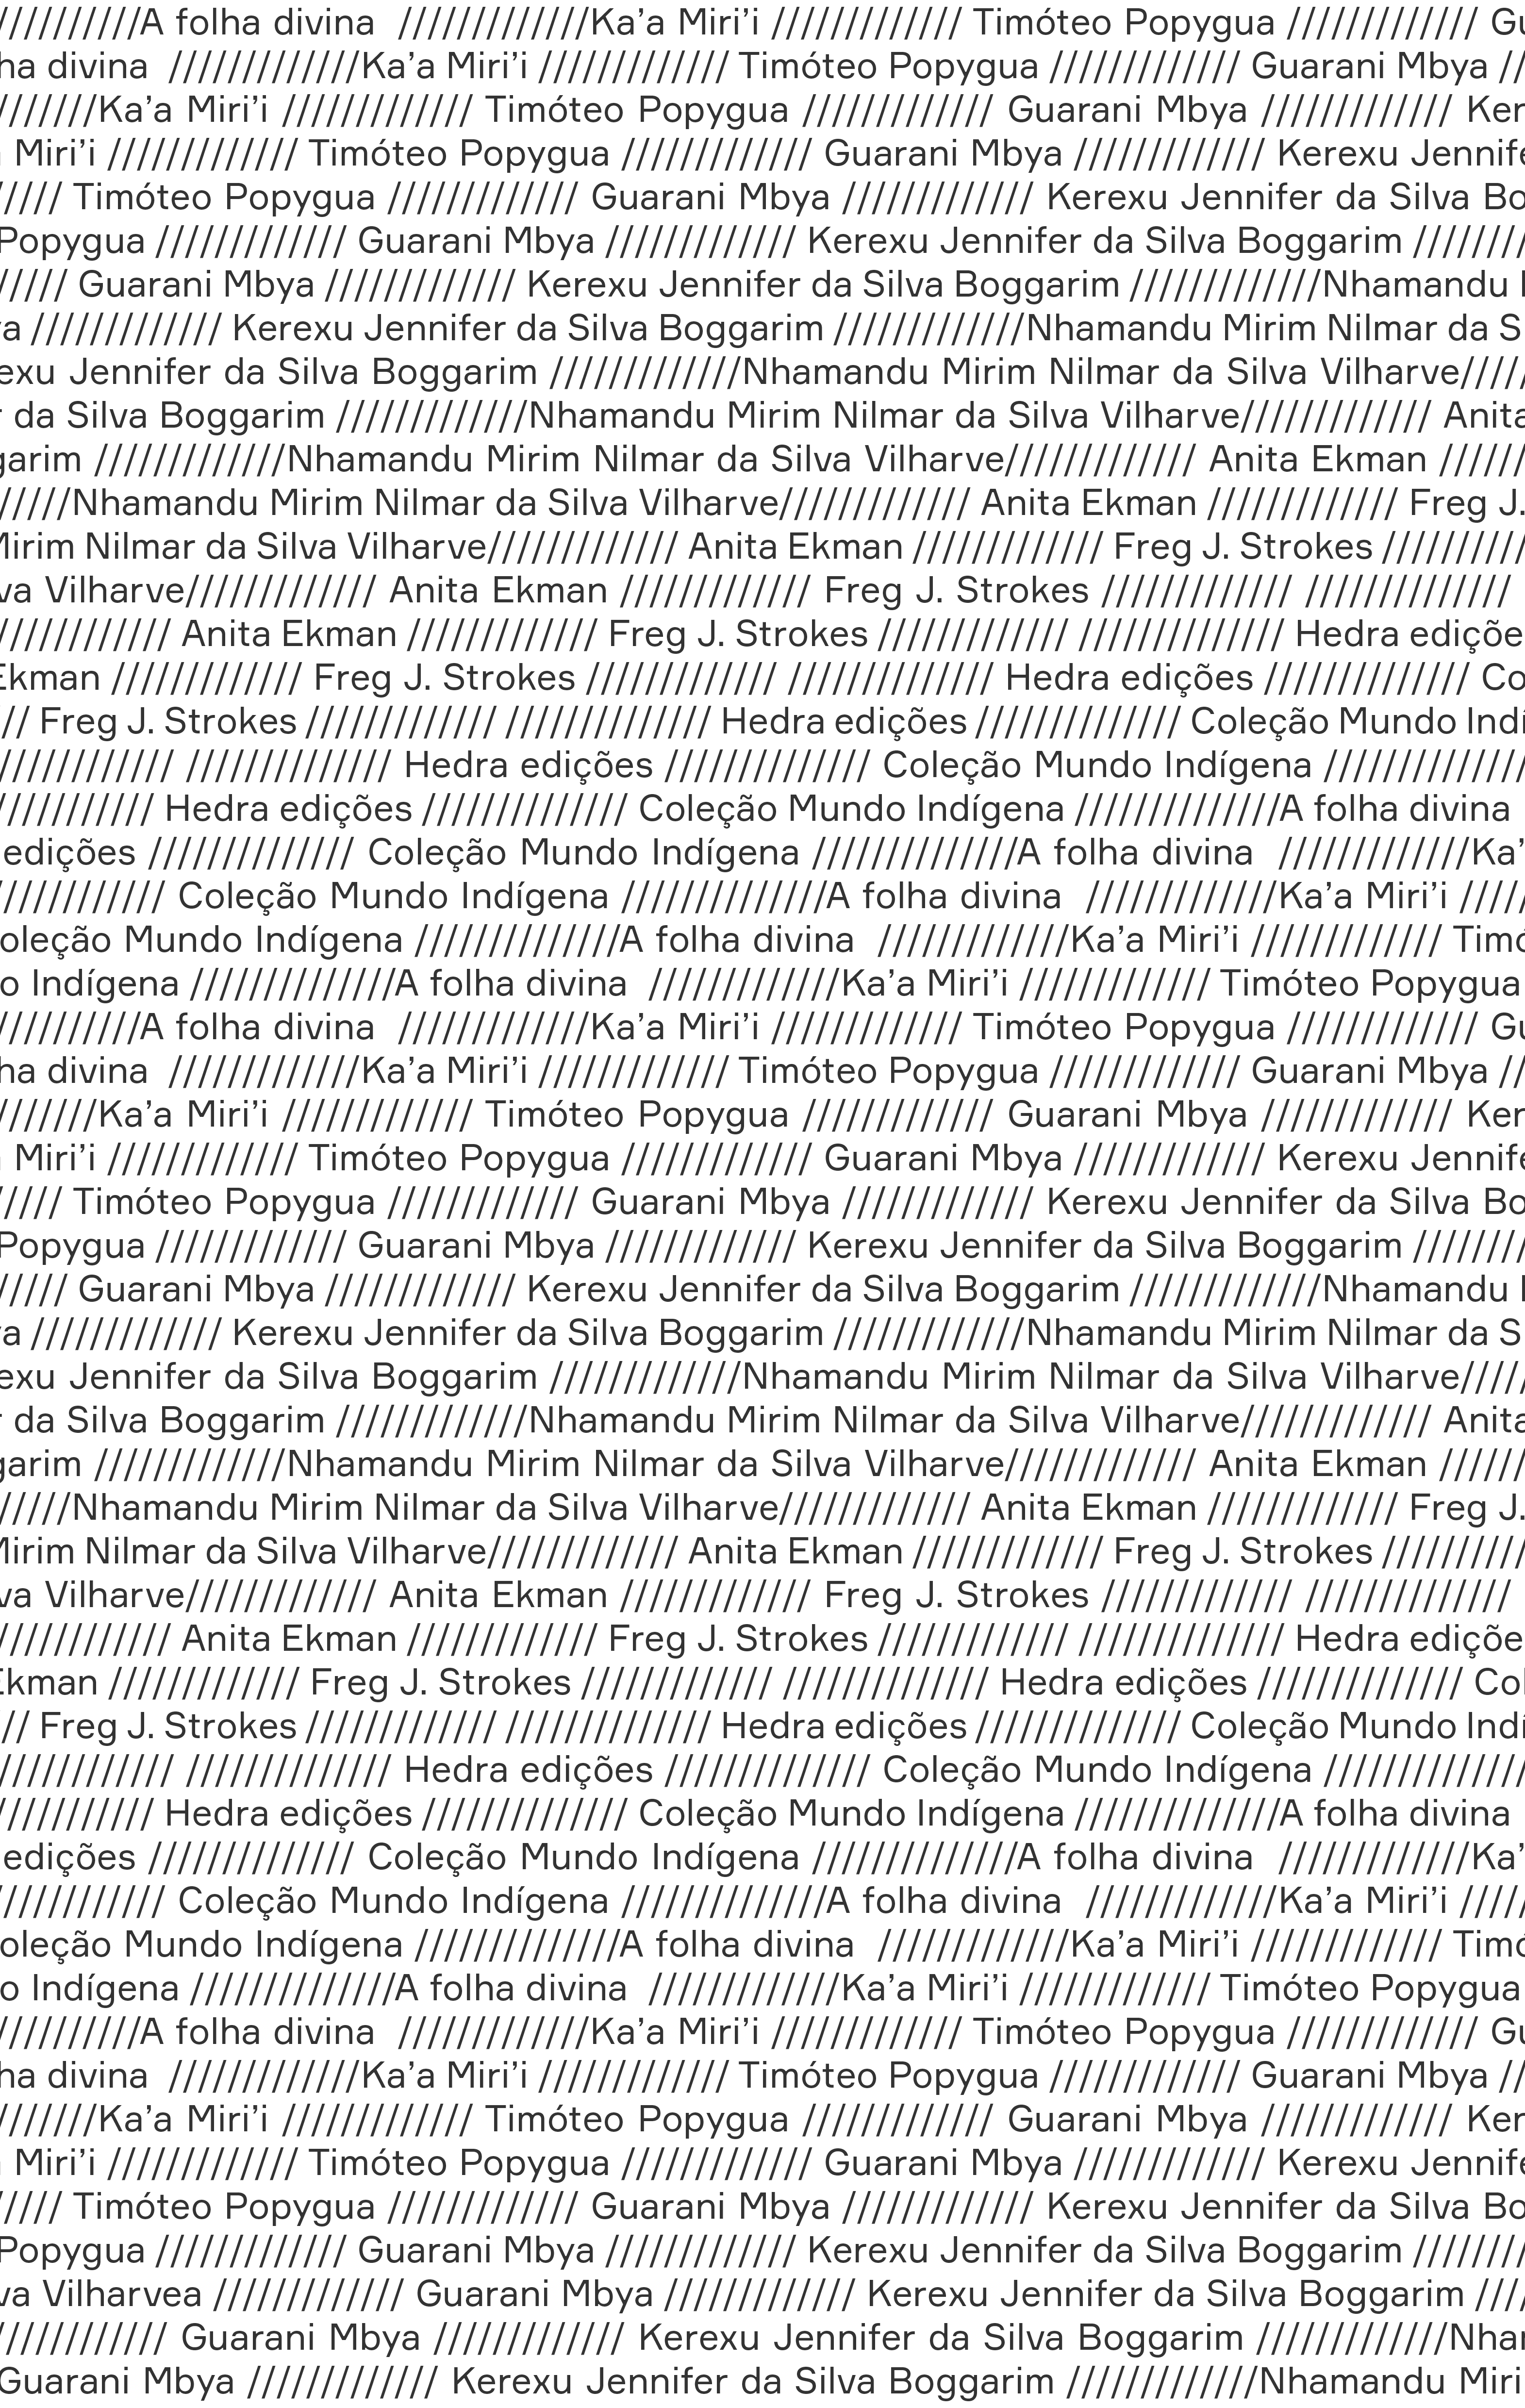
\includegraphics[width=138mm]{./ABERTURA.png}  
\end{textblock*}
\clearpage
\pagebreak

\thispagestyle{empty}
\begin{textblock*}{2.625in}(0pt,0pt)%
\vspace*{-2.4cm}
\hspace*{-2.3cm}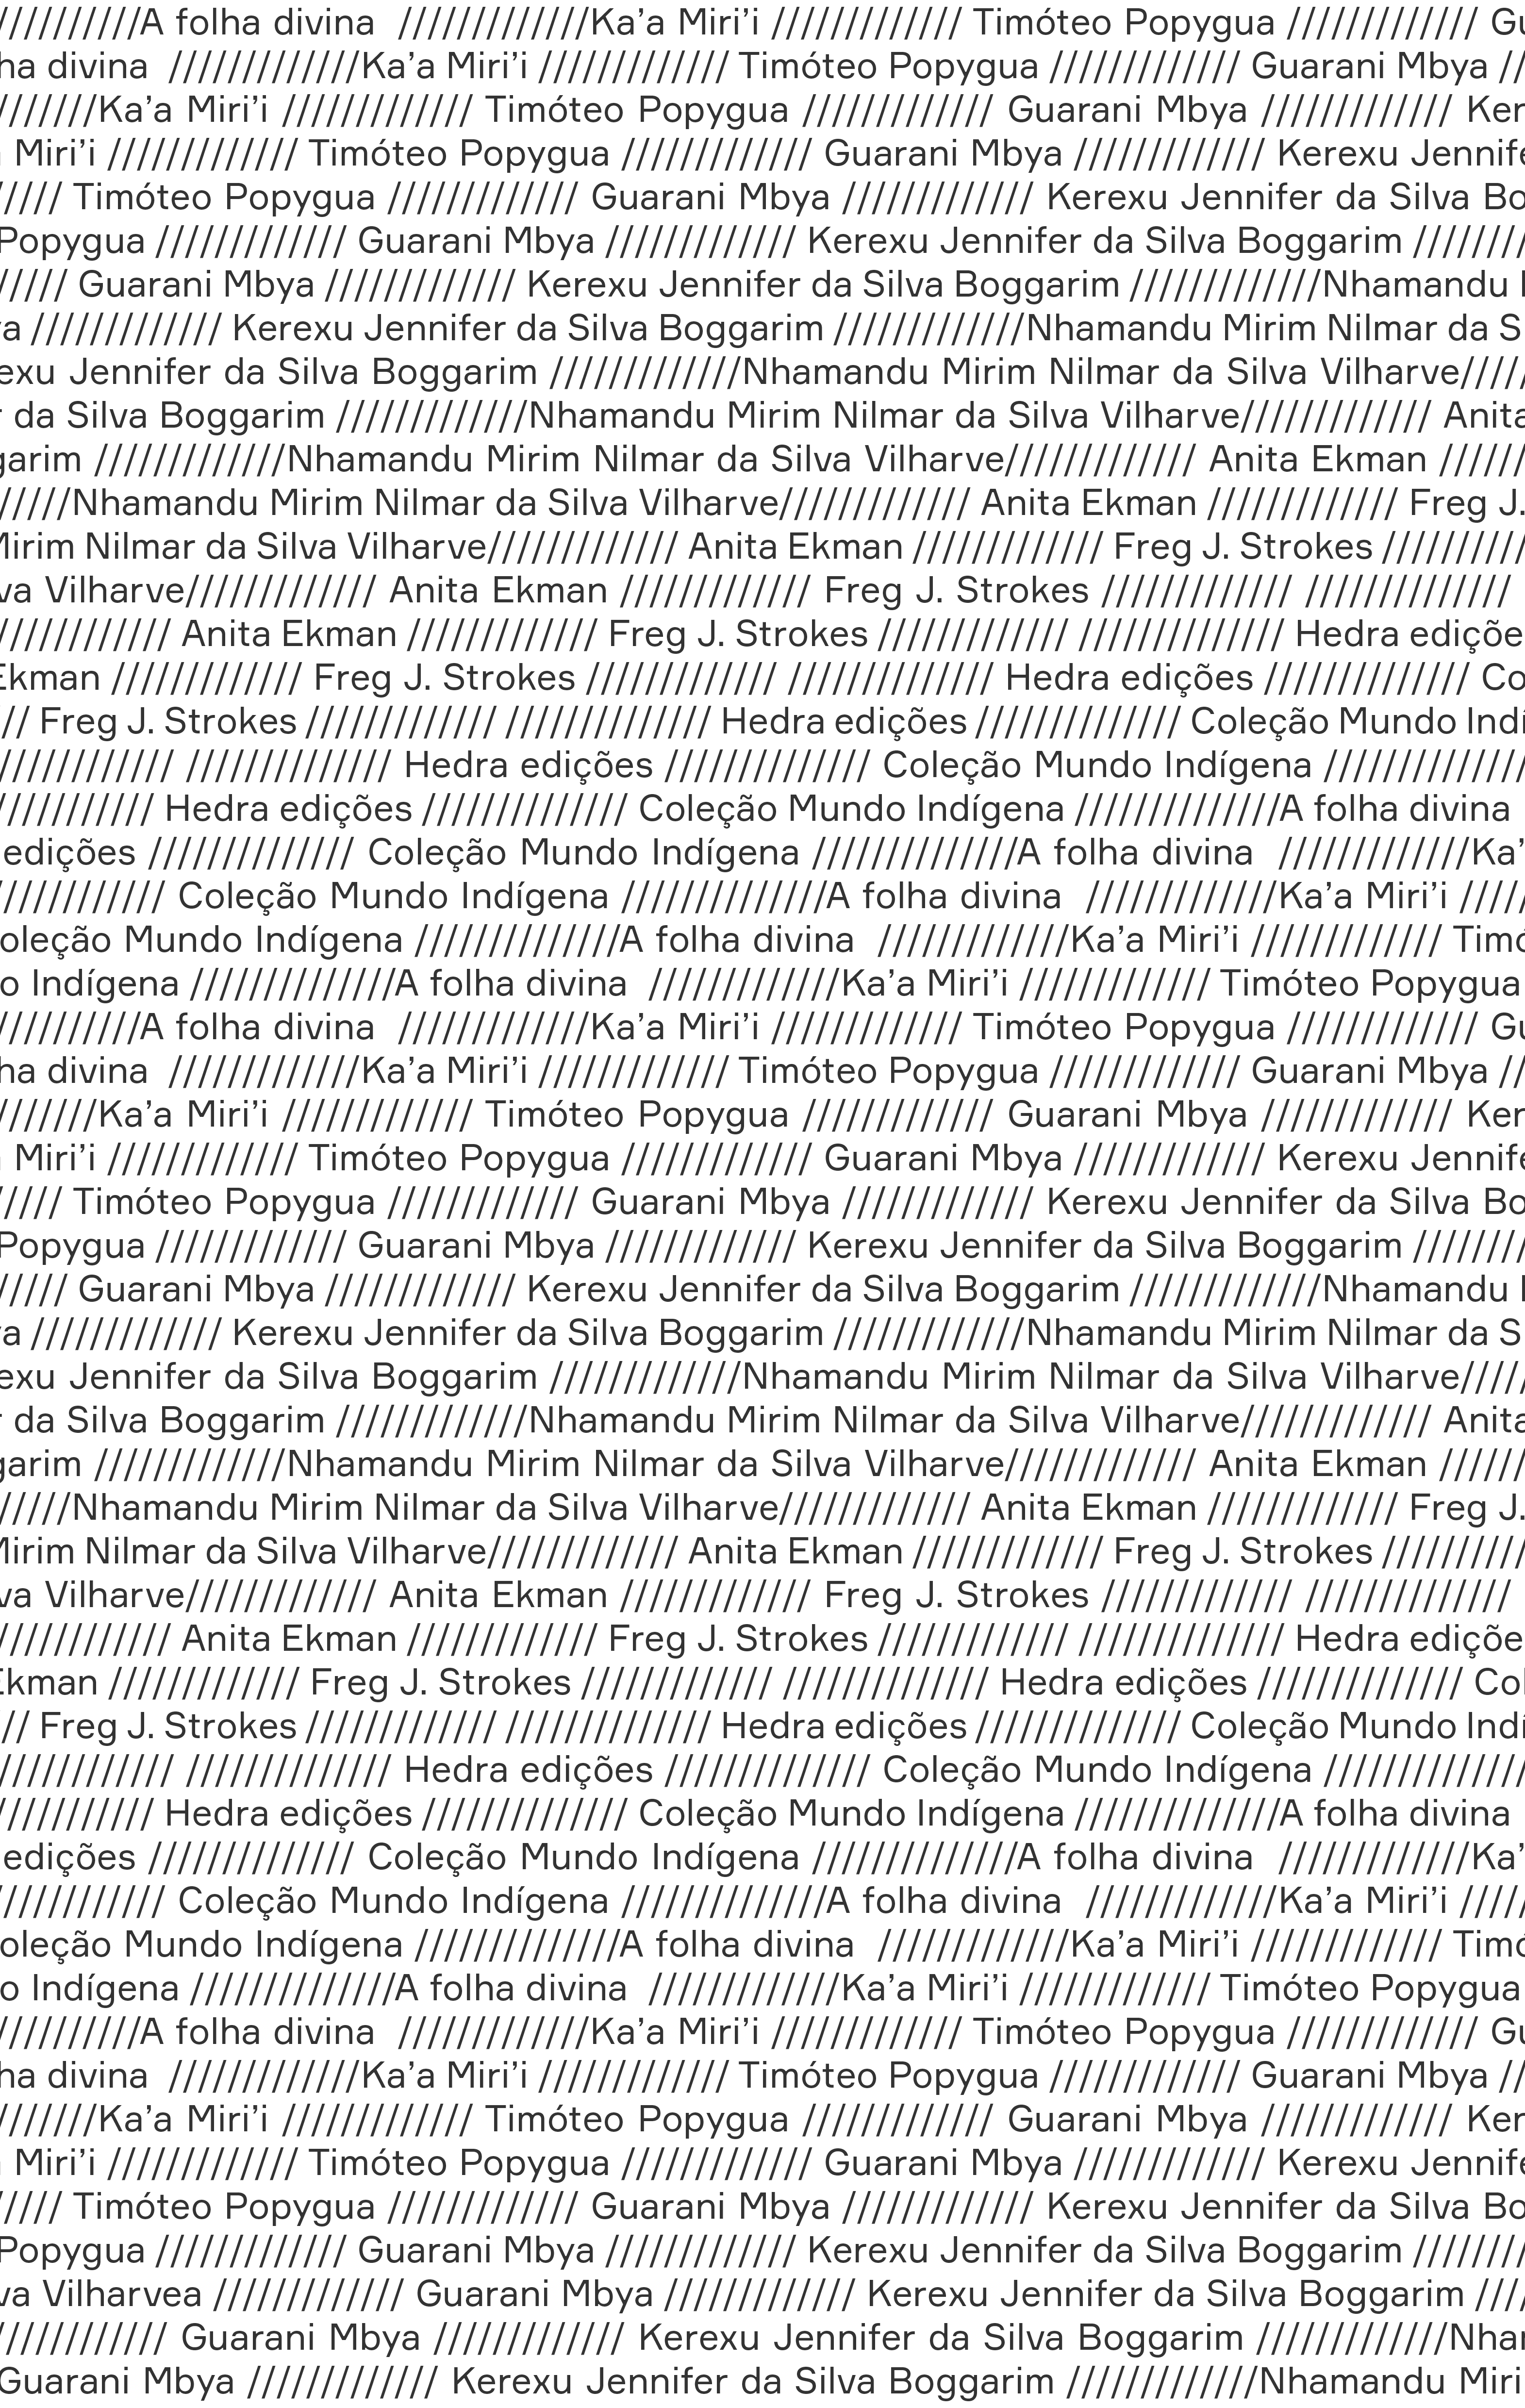
\includegraphics[width=138mm]{./ABERTURA.png}  
\end{textblock*}
\clearpage

\thispagestyle{empty}

% Tamanhos
% \tiny
% \scriptsize
% \footnotesize
% \small 
% \normalsize
% \large 
% \Large 
% \LARGE 
% \huge
% \Huge

% Posicionamento
% \centering 
% \raggedright
% \raggedleft
% \vfill 
% \hfill 
% \vspace{Xcm}   % Colocar * caso esteja no começo de uma página. Ex: \vspace*{...}
% \hspace{Xcm}

% Estilo de página
% \thispagestyle{<<nosso>>}
% \thispagestyle{empty}
% \thispagestyle{plain}  (só número, sem cabeço)
% https://www.overleaf.com/learn/latex/Headers_and_footers

% Compilador que permite usar fonte de sistema: xelatex, lualatex
% Compilador que não permite usar fonte de sistema: latex, pdflatex

% Definindo fontes
% \setmainfont{Times New Roman}  % Todo o texto
% \newfontfamily\avenir{Avenir}  % Contexto

\begingroup\thispagestyle{empty}\vspace*{.05\textheight} 

              {\formular
              \huge
              \noindent
              \textbf{Título}\\
              
              \vspace{-0.5cm}
              
              \noindent{}{\LARGE Título na língua indígena}}
                    
\endgroup
\vfill
\pagebreak       % [Frontistício]
%\newcommand{\linhalayout}[2]{{\tiny\textbf{#1}\quad#2\par}}
\newcommand{\linha}[2]{\ifdef{#2}{\linhalayout{#1}{#2}}{}}

\begingroup\tiny
\parindent=0cm
\thispagestyle{empty}

\textbf{copyright}\quad {Nome do autor}\\
\textbf{edição brasileira©}\quad			 {Hedra \the\year}\\
\textbf{tradução©}\quad			 			 {copyrighttraducao}\\
\textbf{organização©}\quad			 		 {copyrightorganizacao}\\
\textbf{prefácio©}\quad			 			 {copyrightintroducao}\\
\textbf{ilustração©}\quad			 		 {copyrightilustracao}\medskip

\textbf{título original}\quad			 	 {titulooriginal}\\
\textbf{edição consultada}\quad			 	 {edicaoconsultada}\\
\textbf{primeira edição}\quad			 	 {primeiraedicao}\\
\textbf{agradecimentos}\quad			 	 {agradecimentos}\\
\textbf{indicação}\quad			 			 {indicacao}\medskip

\textbf{edição}\quad			 			 {edicao}\\
\textbf{coedição}\quad			 			 {coedicao}\\
\textbf{assistência editorial}\quad			 {assistencia}\\
\textbf{revisão}\quad			 			 {revisao}\\
\textbf{preparação}\quad			 		 {preparacao}\\
\textbf{iconografia}\quad			 		 {iconografia}\\
\textbf{capa}\quad			 				 {capa}\\
\textbf{imagem da capa}\quad			 	 {imagemcapa}\medskip

\textbf{ISBN}\quad			 				 {ISBN}\smallskip

% \hspace{-5pt}\begin{tabular}{ll}
% \textbf{conselho editorial} & Adriano Scatolin,  \\
% 							& Antonio Valverde,  \\
% 							& Caio Gagliardi,    \\
% 							& Jorge Sallum,      \\
% 							& Ricardo Valle,     \\
% 							& Tales Ab'Saber,    \\
% 							& Tâmis Parron      
% \end{tabular}
 

\vfill

\textit{Grafia atualizada segundo o Acordo Ortográfico da Língua\\
Portuguesa de 1990, em vigor no Brasil desde 2009.}\\

\textit{Direitos reservados em língua\\ 
portuguesa somente para o Brasil}\\\medskip

\textsc{editora hedra ltda.}\\
Av.~São Luís, 187, Piso 3, Loja 8 (Galeria Metrópole)\\
01046--912 São Paulo \textsc{sp} Brasil\\
Telefone/Fax +55 11 3097 8304\\\smallskip
editora@hedra.com.br\\
www.hedra.com.br\\
\bigskip
Foi feito o depósito legal.

\endgroup
\pagebreak     % [Créditos]
%!TEX root=./LIVRO.tex
% Tamanhos
% \tiny
% \scriptsize
% \footnotesize
% \small 
% \normalsize
% \large 
% \Large 
% \LARGE 
% \huge
% \Huge

% Posicionamento
% \centering 
% \raggedright
% \raggedleft
% \vfill 
% \hfill 
% \vspace{Xcm}   % Colocar * caso esteja no começo de uma página. Ex: \vspace*{...}
% \hspace{Xcm}

% Estilo de página
% \thispagestyle{<<nosso>>}
% \thispagestyle{empty}
% \thispagestyle{plain}  (só número, sem cabeço)
% https://www.overleaf.com/learn/latex/Headers_and_footers

% Compilador que permite usar fonte de sistema: xelatex, lualatex
% Compilador que não permite usar fonte de sistema: latex, pdflatex

% Definindo fontes
% \setmainfont{Times New Roman}  % Todo o texto
% \newfontfamily\avenir{Avenir}  % Contexto

\begingroup\thispagestyle{empty}\vspace*{.05\textheight} 

              \formular
              \Huge
              \noindent
              \textbf{Título}

              {\brabo\LARGE
              \noindent Autor da silva}
              
              \vfill

  \newfontfamily\minion{Minion Pro}
              \fontsize{30}{40}\selectfont \minion\small
              \noindent Colaborador 1 (\textit{tradução})
              \vspace{0.1cm}

              \noindent Colaborador 2 (\textit{apresentação})

              \vspace{0.5cm}
              
              {\noindent\fontsize{30}{40}\selectfont \minion\small\noindent Xª edição}

              \vfill

              \newfontfamily\timesnewroman{Times New Roman}
              {\noindent\fontsize{30}{40}\selectfont\timesnewroman hedra}
              \smallskip
              
              {\selectfont\minion\small
              \noindent São Paulo \quad\the\year}

\endgroup
\pagebreak
	       % [folha de rosto]

% nothing			is level -3
% \book				is level -2
% \part				is level -1
% \chapter 			is level 0
% \section 			is level 1
% \subsection 		is level 2
% \subsubsection 	is level 3
% \paragraph 		is level 4
% \subparagraph 	is level 5
\setcounter{secnumdepth}{-2}
\setcounter{tocdepth}{0}


\pagebreak
\begingroup \footnotesize \parindent0pt \parskip 5pt \thispagestyle{empty} \vspace*{-0.5\textheight}\mbox{} \vfill
\baselineskip=.92\baselineskip
%!TEX root=./LIVRO.tex
\textbf{Autor} Lorem ipsum dolor sit amet, consectetur adipisicing elit, sed do eiusmod tempor incididunt ut labore et dolore magna aliqua. Ut enim ad minim veniam, quis nostrud exercitation ullamco laboris nisi ut aliquip ex ea commodo consequat. Duis aute irure dolor in reprehenderit in voluptate velit esse cillum dolore eu fugiat nulla pariatur. Excepteur sint occaecat cupidatat non proident, sunt in culpa qui officia deserunt mollit anim id est laborum.

\textbf{Livro} Lorem ipsum dolor sit amet, consectetur adipisicing elit, sed do eiusmod tempor incididunt ut labore et dolore magna aliqua. Ut enim ad minim veniam, quis nostrud exercitation ullamco laboris nisi ut aliquip ex ea commodo consequat. Duis aute irure dolor in reprehenderit in voluptate velit esse cillum dolore eu fugiat nulla pariatur. Excepteur sint occaecat cupidatat non proident, sunt in culpa qui officia deserunt mollit anim id est laborum.

\textbf{Colaborador 1} \lipsum[3]

\textbf{Colaborador 2} \lipsum[4]



\endgroup

\pagebreak
{\begingroup\mbox{}\pagestyle{empty}
\pagestyle{empty} 
\addtocontents{toc}{\protect\thispagestyle{empty}}
\tableofcontents*\clearpage\endgroup}

\input{XXXXXX}
\input{XXXXX}

% Indice remissivo (package: `\usepackage{makeidx}` e no início do arquivi `\makeindex`
% \printindex

% Indice
% \renewcommand{\contentsname}{Índice}
% \setcounter{tocdepth}{3}
% \tableofcontents

% \endnotes

%PEGAR SEMPRE A VERSÃO ATUALIZADA DO REPOSITÓRIO "PUBLICIDADE"
\pagebreak
\blankpage
%\blankAteven
\pagestyle{empty}
\begingroup
\fontsize{7}{8}\selectfont

{\large\textsc{coleção «hedra edições»}}

\begin{enumerate}
\setlength\parskip{4.2pt}
\setlength\itemsep{-1.4mm}
%\item \textit{Poemas da cabana montanhesa}, Saigy\=o
\item \textit{A arte da guerra}, Maquiavel
\item \textit{A conjuração de Catilina}, Salústio
\item \textit{A cruzada das crianças/ Vidas imaginárias}, Marcel Schwob
\item \textit{A filosofia na era trágica dos gregos}, Friedrich Nietzsche
\item \textit{A fábrica de robôs}, Karel Tchápek 
\item \textit{A história trágica do Doutor Fausto}, Christopher Marlowe
\item \textit{A metamorfose}, Franz Kafka
\item \textit{A monadologia e outros textos}, Gottfried Leibniz
\item \textit{A morte de Ivan Ilitch}, Lev Tolstói 
\item \textit{A velha Izerguil e outros contos}, Maksim Górki
\item \textit{A vida é sonho}, Calderón de la Barca
\item \textit{A volta do parafuso}, Henry James
\item \textit{A voz dos botequins e outros poemas}, Paul Verlaine 
\item \textit{A vênus das peles}, Leopold von Sacher{}-Masoch
\item \textit{A última folha e outros contos}, O.\,Henry
\item \textit{Americanismo e fordismo}, Antonio Gramsci
\item \textit{Anarquia pela educação}, Élisée Reclus 
\item \textit{Apologia de Galileu}, Tommaso Campanella 
\item \textit{Arcana C\oe lestia} e \textit{Apocalipsis revelata}, Emanuel Swedenborg
\item \textit{As bacantes}, Eurípides
\item \textit{Autobiografia de uma pulga}, [Stanislas de Rhodes]
\item \textit{Ação direta e outros escritos}, Voltairine de Cleyre
\item \textit{Balada dos enforcados e outros poemas}, François Villon
\item \textit{Carmilla, a vampira de Karnstein}, Sheridan Le Fanu
\item \textit{Carta sobre a tolerância}, John Locke
\item \textit{Contos clássicos de vampiro}, L.\,Byron, B.\,Stoker \& outros
\item \textit{Contos de amor, de loucura e de morte}, Horacio Quiroga
\item \textit{Contos indianos}, Stéphane Mallarmé
\item \textit{Cultura estética e liberdade}, Friedrich von Schiller
\item \textit{Cântico dos cânticos}, [Salomão]
\item \textit{Dao De Jing}, Lao Zi
\item \textit{Discursos ímpios}, Marquês de Sade
\item \textit{Dissertação sobre as paixões}, David Hume
\item \textit{Diário de um escritor (1873)}, Fiódor Dostoiévski
\item \textit{Diário parisiense e outros escritos}, Walter Benjamin
\item \textit{Diários de Adão e Eva}, Mark Twain
\item \textit{Don Juan}, Molière
\item \textit{Dos novos sistemas na arte}, Kazimir Maliévitch
\item \textit{Educação e sociologia}, Émile Durkheim
\item \textit{Édipo Rei}, Sófocles
\item \textit{Elogio da loucura}, Erasmo de Rotterdam
\item \textit{Émile e Sophie ou os solitários}, Jean-Jacques Rousseau 
\item \textit{Emília Galotti}, Gotthold Ephraim Lessing
\item \textit{Entre camponeses}, Errico Malatesta
\item \textit{Ernestine ou o nascimento do amor}, Stendhal
\item \textit{Escritos revolucionários}, Errico Malatesta
\item \textit{Escritos sobre arte}, Charles Baudelaire
\item \textit{Escritos sobre literatura}, Sigmund Freud
\item \textit{Eu acuso!}, Zola/\,\textit{O processo do capitão Dreyfus}, Rui Barbosa
\item \textit{Explosão: romance da etnologia}, Hubert Fichte
\item \textit{Fedro}, Platão
\item \textit{Feitiço de amor e outros contos}, Ludwig Tieck
\item \textit{Flossie, a Vênus de quinze anos}, [Swinburne]
\item \textit{Fábula de Polifemo e Galateia e outros poemas}, Góngora
\item \textit{Fé e saber}, Georg W.\,F.\,Hegel
\item \textit{Gente de Hemsö}, August Strindberg 
\item \textit{Hawthorne e seus musgos}, Melville
\item \textit{Hino a Afrodite e outros poemas}, Safo de Lesbos 
\item \textit{História da anarquia (vol.\,\textsc{ii})}, Max Nettlau
\item \textit{História da anarquia (vol.\,\textsc{i})}, Max Nettlau
\item \textit{Imitação de Cristo}, Tomás de Kempis
\item \textit{Incidentes da vida de uma escrava}, Harriet Jacobs
\item \textit{Inferno}, August Strindberg
\item \textit{Investigação sobre o entendimento humano}, David Hume
\item \textit{Jazz rural}, Mário de Andrade
\item \textit{Jerusalém}, William Blake
\item \textit{Joana d'Arc}, Jules Michelet
\item \textit{Lira grega}, Giuliana Ragusa (org.)
\item \textit{Lisístrata}, Aristófanes 
\item \textit{Ludwig Feuerbach e o fim da filosofia clássica alemã}, Friederich Engels
\item \textit{Manifesto comunista}, Karl Marx e Friederich Engels
\item \textit{Memórias do subsolo}, Fiódor Dostoiévski
\item \textit{Metamorfoses}, Ovídio
\item \textit{Micromegas e outros contos}, Voltaire
\item \textit{Narrativa de William W.\,Brown, escravo fugitivo}, William Wells Brown
\item \textit{Nascidos na escravidão: depoimentos norte-americanos}, \textsc{wpa}
\item \textit{No coração das trevas}, Joseph Conrad
\item \textit{Noites egípcias e outros contos}, Aleksandr Púchkin
\item \textit{O casamento do Céu e do Inferno}, William Blake
\item \textit{O cego e outros contos}, \textsc{d.\,h}.\,Lawrence
\item \textit{O chamado de Cthulhu}, \textsc{h.\,p.}\,lovecraft
\item \textit{O contador de histórias e outros textos}, Walter Benjamin
\item \textit{O corno de si próprio e outros contos}, Marquês de Sade
\item \textit{O destino do erudito}, Johann Fichte
\item \textit{O estranho caso do dr.\,Jekyll e Mr. Hyde}, Robert Louis Stevenson
\item \textit{O fim do ciúme e outros contos}, Marcel Proust
\item \textit{O indivíduo, a sociedade e o Estado, e outros ensaios}, Emma Goldman
\item \textit{O ladrão honesto e outros contos}, Fiódor Dostoiévski
\item \textit{O livro de Monelle}, Marcel Schwob
\item \textit{O mundo ou tratado da luz}, René Descartes
\item \textit{O novo Epicuro: as delícias do sexo}, Edward Sellon
\item \textit{O pequeno Zacarias, chamado Cinábrio}, \textsc{e.\,t.\,a.}\,Hoffmann
\item \textit{O primeiro Hamlet}, William Shakespeare
\item \textit{O princípio anarquista e outros ensaios}, Piotr Kropotkin
\item \textit{O princípio do Estado e outros ensaios}, Mikhail Bakunin
\item \textit{O príncipe}, Maquiavel
\item \textit{O que eu vi, o que nós veremos}, Santos-Dumont
\item \textit{O retrato de Dorian Gray}, Oscar Wilde
\item \textit{O sobrinho de Rameau}, Diderot
\item \textit{Ode ao Vento Oeste e outros poemas}, \textsc{p.\,b.}\,Shelley
\item \textit{Ode sobre a melancolia e outros poemas}, John Keats
\item \textit{Odisseia}, Homero
\item \textit{Oliver Twist}, Charles Dickens
\item \textit{Origem do drama barroco}, Walter Benjamin
\item \textit{Os sofrimentos do jovem Werther}, Goethe
\item \textit{Os sovietes traídos pelos bolcheviques}, Rudolf Rocker
\item \textit{Para serem lidas à noite}, Ion Minulescu
\item \textit{Pensamento político de Maquiavel}, Johann Fichte
\item \textit{Pequeno-burgueses}, Maksim Górki
\item \textit{Pequenos poemas em prosa}, Charles Baudelaire
\item \textit{Perversão: a forma erótica do ódio}, Robert Stoller
\item \textit{Poemas}, Lord Byron
\item \textit{Poesia basca: das origens à Guerra Civil} 
\item \textit{Poesia catalã: das origens à Guerra Civil} 
\item \textit{Poesia espanhola: das origens à Guerra Civil} 
\item \textit{Poesia galega: das origens à Guerra Civil} 
\item \textit{Pr\ae terita}, John Ruskin
\item \textit{Primeiro livro dos Amores}, Ovídio
\item \textit{Rashômon e outros contos}, Ryūnosuke Akutagawa
\item \textit{Revolução e liberdade: cartas de 1845 a 1875}, Mikhail Bakunin
\item \textit{Robinson Crusoé}, Daniel Defoe
\item \textit{Romanceiro cigano}, Federico García Lorca
\item \textit{Sagas}, August Strindberg
\item \textit{Sobre a amizade e outros diálogos}, Jorge Luis Borges e Osvaldo Ferrari
\item \textit{Sobre a filosofia e outros diálogos}, Jorge Luis Borges e Osvaldo Ferrari
\item \textit{Sobre a filosofia e seu método (Parerga e paralipomena)} (v.\textsc{ii}, t.\textsc{i}), Arthur Schopenhauer 
\item \textit{Sobre a liberdade}, Stuart Mill
\item \textit{Sobre a utilidade e a desvantagem da histório para a vida}, Friedrich Nietzsche
\item \textit{Sobre a ética (Parerga e paralipomena)} (v.\textsc{ii}, t.\textsc{ii}), Arthur Schopenhauer 
\item \textit{Sobre anarquismo, sexo e casamento}, Emma Goldman
\item \textit{Sobre o riso e a loucura}, [Hipócrates]
\item \textit{Sobre os sonhos e outros diálogos}, Jorge Luis Borges e Osvaldo Ferrari
\item \textit{Sobre verdade e mentira}, Friedrich Nietzsche
\item \textit{Sonetos}, William Shakespeare
\item \textit{Sátiras, fábulas, aforismos e profecias}, Leonardo da Vinci
\item \textit{Teleny, ou o reverso da medalha}, Oscar Wilde
\item \textit{Teogonia}, Hesíodo
\item \textit{Trabalhos e dias}, Hesíodo
\item \textit{Triunfos}, Petrarca
\item \textit{Um anarquista e outros contos}, Joseph Conrad
\item \textit{Viagem aos Estados Unidos}, Alexis de Tocqueville
\item \textit{Viagem em volta do meu quarto}, Xavier de Maistre 
\item \textit{Viagem sentimental}, Laurence Sterne
\end{enumerate}

% {\large\textsc{coleção «metabiblioteca»}}

% \begin{enumerate}
% \setlength\parskip{4.2pt}
% \setlength\itemsep{-1.4mm}
% \item \textit{A carteira de meu tio}, Joaquim Manuel de Macedo
% \item \textit{A cidade e as serras}, Eça de Queirós
% \item \textit{A escrava}, Maria Firmina dos Reis
% \item \textit{A família Medeiros}, Júlia Lopes de Almeida 
% \item \textit{A pele do lobo e outras peças}, Artur Azevedo
% \item \textit{Auto da barca do inferno}, Gil Vicente
% \item \textit{Bom crioulo}, Adolfo Caminha
% \item \textit{Cartas a favor da escravidão}, José de Alencar
% \item \textit{Contos e novelas}, Júlia Lopes de Almeida
% \item \textit{Crime}, Luiz Gama
% \item \textit{Democracia}, Luiz Gama
% \item \textit{Direito}, Luiz Gama
% \item \textit{Elixir do pajé: poemas de humor, sátira e escatologia}, Bernardo Guimarães
% \item \textit{Eu}, Augusto dos Anjos
% \item \textit{Farsa de Inês Pereira}, Gil Vicente
% \item \textit{Helianto}, Orides Fontela
% \item \textit{História da província Santa Cruz}, Gandavo
% \item \textit{Iracema}, José de Alencar
% \item \textit{Liberdade}, Luiz Gama
% \item \textit{Mensagem}, Fernando Pessoa
% \item \textit{Meridiano 55}, Flávio de Carvalho
% \item \textit{O Ateneu}, Raul Pompeia
% \item \textit{O cortiço}, Aluísio Azevedo
% \item \textit{O desertor}, Silva Alvarenga
% \item \textit{Oração aos moços}, Rui Barbosa
% \item \textit{Pai contra mãe e outros contos}, Machado de Assis
% \item \textit{Poemas completos de Alberto Caeiro}, Fernando Pessoa
% \item \textit{Teatro de êxtase}, Fernando Pessoa
% \item \textit{Transposição}, Orides Fontela
% \item \textit{Tratado descritivo do Brasil em 1587}, Gabriel Soares de Sousa
% \item \textit{Tratados da terra e gente do Brasil}, Fernão Cardim 
% \item \textit{Utopia Brasil}, Darcy Ribeiro
% \item \textit{Índice das coisas mais notáveis}, Antônio Vieira
% \end{enumerate}

% \medskip
% {\large\textsc{coleção «que horas são?»}}

% \begin{enumerate}
% \setlength\parskip{4.2pt}
% \setlength\itemsep{-1.4mm}
% \item \textit{8/1: A rebelião dos manés}, Pedro Fiori Arantes, Fernando Frias e Maria Luiza Meneses
% \item \textit{A linguagem fascista}, Carlos Piovezani \& Emilio Gentile
% \item \textit{A sociedade de controle}, J.\,Souza; R.\,Avelino; S.\,Amadeu (orgs.)
% \item \textit{Ativismo digital hoje}, R.\,Segurado; C.\,Penteado; S.\,Amadeu (orgs.)
% \item \textit{Crédito à morte}, Anselm Jappe
% \item \textit{Descobrindo o Islã no Brasil}, Karla Lima
% \item \textit{Desinformação e democracia}, Rosemary Segurado
% \item \textit{Dilma Rousseff e o ódio político}, Tales Ab'Sáber
% \item \textit{Labirintos do fascismo} (v.\textsc{iii}), João Bernardo
% \item \textit{Labirintos do fascismo} (v.\textsc{ii}), João Bernardo
% \item \textit{Labirintos do fascismo} (v.\textsc{iv}), João Bernardo
% \item \textit{Labirintos do fascismo} (v.\textsc{i}), João Bernardo
% \item \textit{Labirintos do fascismo} (v.\textsc{vi}), João Bernardo
% \item \textit{Labirintos do fascismo} (v.\textsc{v}), João Bernardo
% \item \textit{Lugar de negro, lugar de branco?}, Douglas Rodrigues Barros
% \item \textit{Lulismo, carisma pop e cultura anticrítica}, Tales Ab'Sáber
% \item \textit{Machismo, racismo, capitalismo identitário}, Pablo Polese
% \item \textit{Michel Temer e o fascismo comum}, Tales Ab'Sáber
% \item \textit{O quarto poder: uma outra história}, Paulo Henrique Amorim
% \item \textit{Universidade, cidade e cidadania}, Franklin Leopoldo e Silva
% \end{enumerate}

% \medskip
% {\large\textsc{coleção «mundo indígena»}}

% \begin{enumerate}
% \setlength\parskip{4.2pt}
% \setlength\itemsep{-1.4mm}
% \item \textit{A folha divina}, Timóteo Verá Tupã Popygua
% \item \textit{A mulher que virou tatu}, Eliane Camargo
% \item \textit{A terra uma só}, Timóteo Verá Tupã Popygua
% \item \textit{A árvore dos cantos}, Pajés Parahiteri
% \item \textit{Cantos dos animais primordiais}, Ava Ñomoandyja Atanásio Teixeira
% \item \textit{Crônicas de caça e criação}, Uirá Garcia
% \item \textit{Círculos de coca e fumaça}, Danilo Paiva Ramos
% \item \textit{Nas redes guarani}, Valéria Macedo \& Dominique Tilkin-Gallois
% \item \textit{Não havia mais homens}, Luciana Storto
% \item \textit{O surgimento da noite}, Pajés Parahiteri
% \item \textit{O surgimento dos pássaros}, Pajés Parahiteri
% \item \textit{Os Aruaques}, Max Schmidt
% \item \textit{Os cantos do homem-sombra}, Patience Epps e Danilo Paiva Ramos
% \item \textit{Os comedores de terra}, Pajés Parahiteri
% \item \textit{Xamanismos ameríndios}, A.\,Barcelos Neto, L.\,Pérez Gil \& D.\,Paiva Ramos
% \end{enumerate}

% \medskip
% {\large\textsc{coleção «ecopolítica»}}

% \begin{enumerate}
% \setlength\parskip{4.2pt}
% \setlength\itemsep{-1.4mm}
% \item \textit{Anarquistas na América do Sul}, E.\,Passetti, S.\,Gallo; A.\,Augusto  (orgs.)
% \item \textit{Ecopolítica}, E.\,Passetti; A.\,Augusto; B.\,Carneiro; S.\,Oliveira, T.\,Rodrigues  (orgs.)
% \item \textit{Pandemia e anarquia}, E.\,Passetti; J.\,da Mata; J.\,Ferreira  (orgs.)
% \end{enumerate}

% % \medskip
% % {\large\textsc{coleção <<anarc>>}}

% % \begin{enumerate}
% % \setlength\parskip{4.2pt}
% % \setlength\itemsep{-1.4mm}
% % \item \textit{Anarquia pela educação}, Élisée Reclus 
% % \item \textit{Ação direta e outros escritos}, Voltairine de Cleyre
% % \item \textit{Entre camponeses}, Errico Malatesta
% % \item \textit{Escritos revolucionários}, Errico Malatesta
% % \item \textit{História da anarquia (vol.\,\textsc{ii})}, Max Nettlau
% % \item \textit{História da anarquia (vol.\,\textsc{i})}, Max Nettlau
% % \item \textit{O indivíduo, a sociedade e o Estado, e outros ensaios}, Emma Goldman
% % \item \textit{O princípio anarquista e outros ensaios}, Piotr Kropotkin
% % \item \textit{O princípio do Estado e outros ensaios}, Mikhail Bakunin
% % \item \textit{Os sovietes traídos pelos bolcheviques}, Rudolf Rocker
% % \item \textit{Revolução e liberdade: cartas de 1845 a 1875}, Mikhail Bakunin
% % \item \textit{Sobre anarquismo, sexo e casamento}, Emma Goldman
% % \end{enumerate}

% % \medskip
% % {\large\textsc{coleção <<narrativas da escravidão>>}}

% % \begin{enumerate}
% % \setlength\parskip{4.2pt}
% % \setlength\itemsep{-1.4mm}
% % \item \textit{Incidentes da vida de uma escrava}, Harriet Jacobs
% % \item \textit{Narrativa de William W.\,Brown, escravo fugitivo}, William Wells Brown
% % \item \textit{Nascidos na escravidão: depoimentos norte-americanos}, \textsc{wpa}
% % \end{enumerate}


 \pagebreak	   % [lista de livros publicados]
%!TEX root=./LIVRO.tex
\pagebreak

\ifodd\thepage\blankpage\fi

\mbox{}\vfill


\begin{center}
		\begin{minipage}{.7\textwidth}\tiny\noindent{}
		\centering\tiny
		Adverte-se aos curiosos que se imprimiu este 
		livro
		% na gráfica Meta Brasil, 
		em \today{} em papel pólen soft, em tipologia Minion Pro e Formular, 
		com diversos sofwares livres, 
		entre eles, Lua\LaTeX, git.\\ 
		\ifdef{\RevisionInfo{}}{\par(v.\,\RevisionInfo)}{}\medskip\\\
		\adforn{64}
		\end{minipage}
\end{center}		   % [colofon]